\chapter{Joint SegNet and statistical techniques for Improving the Border Cut-Off}

\section{Introduction}
This chapter focuses on the implementation of a standard deep learning algorithm called SegNet and improving its border cut-off accuracy using statistical techniques (Otsu, LBPC). The disadvantages of deep learning techniques are highlighted and the importance of an accurate border cut-off is explored for the analysis of ABCD rules.

\section{Background}
%Discuss the ABCD rule techniques and how border is better with a tighter border rather than segmentation from techniques including SegNet
Segmentation plays a crucial role in correctly identifying melanoma. The accurate recognition of melanoma is a challenging task due to the contrast between lesions and skin, including visual similarities between melanoma and non-melanoma skin lesions\cite{Li2018a}. For example, classification tasks are improved by separating the lesion from healthy skin ensuring that only relevant sections of the lesion are classified\cite{Albahli2020, bi2019}. The goal of producing segmentation techniques is to simplify and transform the representation of images into a more meaningful form for analysis, which is essential for precise representations of melanoma lesions\cite{Masood2013a}. This essentially leads to a more effective diagnosis by identifying key features that indicate malignancy\cite{Ali2020a}. Overall segmentation is vital for the accurate and reliable analysis of melanoma.

Accurate segmentation is important for the analysis of ABCD rules\cite{Lee2020}. Especially for the analysis of border features\cite{Pereira2020, Kaya2016} that rely on convexes and indents. The irregularity of borders is a key feature in distinguishing melanoma from benign lesions, and the exact identification of irregular borders from melanoma skin lesions is clinically significant\cite{patil2021}. An accurate border cut-off is also important for the analysis of asymmetry and colour which both classify the colour of the skin lesion. An accurate border is also essential to analysing lesions by preventing skin from accidentally being calculated in the process, ruining the accuracy. It's important to note that many of the ABCD rules algorithms are statistical and sensitive to incorrect segmentations.

\subsection{Significance of Border cut-off}
The border cut-off sometimes referred to as an expert border is essentially a precise border that captures the edges between the skin and skin lesion. This is shown further in figure\ref{seg-expert} from the ISIC 2018 dataset that has a mixture of approximate and expert border types. 

%Show example of borders and expert borders
\begin{figure}[]
    \centering
    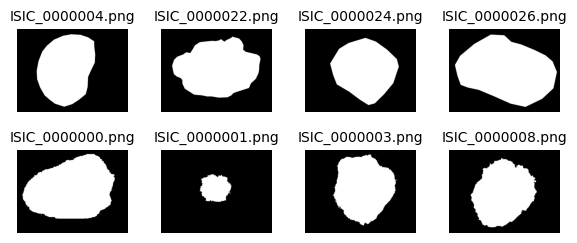
\includegraphics[scale=0.9]{images/segmentation/seg-expert-approx.png}
    \caption{This figure shows examples of different styles of segmentation in the ISIC 2018 dataset with approximate segmentation masks on the top row and expert segmentation masks on the bottom.}\label{seg-expert}
\end{figure}

Many of the deep learning algorithms produce approximate borders; a rough area around the lesion with no border cut-off for the lesion. The ABCD rules techniques rely on border cut-offs. For example, colour analysis relies on removing any remaining skin colour and the border relies on indents and convexes that are not present in approximate borders.

Essentially, for the analysis of ABCD rules the use of deep learning SegNet is not effective enough for their analysis. Therefore, statistical techniques (Otsu, LBPC) are tested to adjust the border as a joint technique.

\subsection{Methodology}
%Explain training parameters
In evaluating the effectiveness of the trained model, several training parameters are commonly used. These parameters serve as quantitative measures to assess the performance of models. The following parameters are utilised:

\begin{itemize}
    \item Loss: The loss function is a parameter used to measure the inconsistency between the predicted segmentation and the ground truth. Loss is typically minimised as the model is trained through the optimisation algorithm including Adam or stochastic gradient descent (SGD).

    \item Recall: The recall function otherwise known as sensitivity evaluates the ability of the model to correctly identify instances within an image. For example, it is calculated as a true positive to the sum of true positives and false negatives. A high recall value means that the model is effective at capturing the relevant objects in the image.

    \item Accuracy: The accuracy is a fundamental metric that measures the overall correctness of the model's classification. It is calculated by the number of correct predictions to the total number of predictions. Accuracy tends to be ineffective in analysing unbalanced datasets.

    \item The precision quantifies the accuracy of the model's positive predictions. It is calculated as the true positive to the sum of true positives and false positives. A high precision indicates that the model has a low risk of producing false positive predictions.

    \item Dice Coefficient: The dice coefficient that is also known as F1 score is a metric that combines precision and recall into a single value. It is calculated as the harmonic mean of precision and recall. This provides a balanced assessment of general model performance in segmenting images.

    \item Jaccard Index: The Jaccard index or Intersection over Union (IoU) measures the similarity between the predicted segmentation and ground truth. It is calculated with the intersection of the predicted and ground truth regions to the union, providing the model's segmentation accuracy.
\end{itemize}

These parameters are a collective evaluation of the SegNet model's performance in image segmentation.

%Out of 2,594 images ... are added to the approximate dataset of ... because they do not have expert borders. However because of the number of images needed to train the algorithms. Considering the deep learning algorithms only produce a rough border they are tested against the approximate borders in the ISIC 2018 dataset. This should allow for a better comparison of the techniques.

%There are various deep learning segmentation approaches\cite{Albahli2020} and CNN techniques\cite{yu2017}. These highlight the significance of advanced technologies for accurate segmentation and detection of melanoma.

\section{Semantic Pixel-Wise Segmentation (SegNet)}
Semantic Pixel-wise segmentation termed SegNet is a deep convolutional encoder-decoder architecture designed for the automatic segmentation of images. It was originally developed in 2015 by Badrinarayanan et al.\cite{Badrinarayanan2017} and has shown promising results for various segmentation tasks including those in the medical field. SegNet has been used in a variety of applications in the medical field including dental imaging\cite{kwak2020}, liver tumour segmentation\cite{Priyadarsini2022}, and many others. It is known for its efficiency in terms of memory and computational time and is known for being more memory efficient than other architectures including U-Net\cite{Mirzazade2021}. Further developments have been made in upgrading SegNet into different versions including Bayesian SegNet\cite{Dhanagopal2022}, and transfer learning using VGG-SegNet\cite{daniel2022}, and ResNet-SegNet\cite{mohd2020}, with differences in the encoder and decoder layers.

The engine consists of an encoder network with identical 13 convolutional layers. The idea of SegNet is to perform pixel-wise classification by assigning each pixel in an image to a specific class or category. This is achieved through a deep convolutional encoder-decoder architecture, which allows for robust semantic pixel-wise labelling.

Semantic pixel-wise segmentation (SegNet) is a machine learning architecture utilizing a deep, fully convolutional neural network (DCNN). This network requires training from ground truth and pre-segmented images for automatic segmentation. SegNet consists of encoding layers, decoding layers, and a pixel-wise classification layer. The encoder layers consist of 3$\times$3 convolutions (including batch normalization and ReLU), and pre-trained filters for classifying features. After some convolutions, the data is down-sampled using a 2$\times$2 pooling layer. Next, decoding layers consist of up-sampling, followed by 3$\times$3 convolutions. Finally, the pixel-wise classification uses a softmax layer to represent each pixel between 0 and 1 based on the previous layers, generating a segmentation mask.

%Show SegNet model
\begin{figure}[]
    \centering
    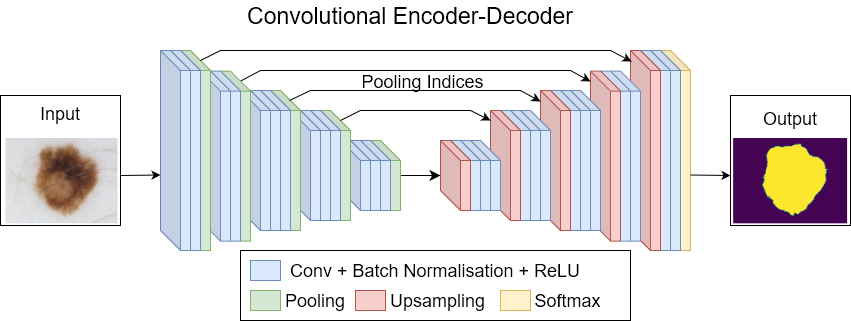
\includegraphics[scale=0.5]{images/segmentation/segnet-arch.png}
    \caption{This diagram shows the SegNet architecture.}\label{SegNet-arch}
\end{figure}

%Mention training parameters
The optimisation model Adam was utilised with learning rate of $0.01$ and a loss of binary cross-entropy. Adam was designed to replace stochastic gradient descent (SGD) because it is generally better than other models and has a faster computational time. 

\begin{figure}[]
    \centering
    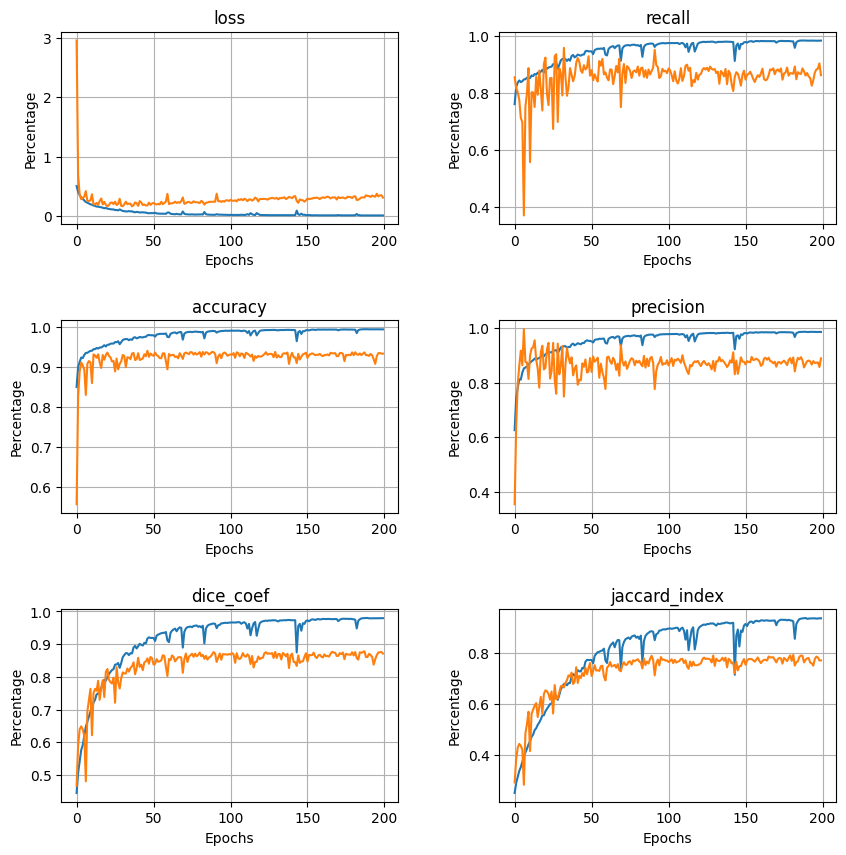
\includegraphics[scale=0.7]{images/segmentation/SegNet-results.png}
    \caption{}\label{SegNet-results}
\end{figure}

%Share results
After training the model using parameters and 100 epochs the trained model has the following metrics, shown in figure \ref{SegNet-results}. In the diagram blue represents training data making up 80\% of the overall data and orange is the validation data making 20\%. All the training parameters increase to above a certain percentage, and although the validation appears to have stopped increasing it isn't decreasing. If it was decreasing it would demonstrate overfitting.

\begin{figure}[]
    \centering
    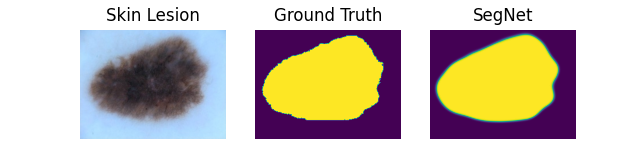
\includegraphics[scale=0.8]{images/segmentation/SegNet-1.png}
    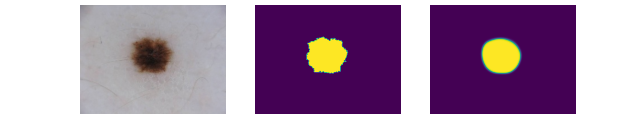
\includegraphics[scale=0.8]{images/segmentation/SegNet-2.png}
    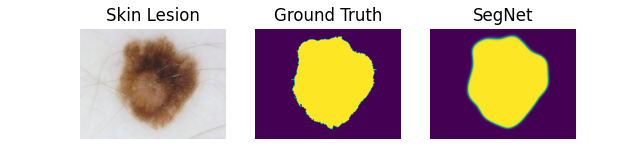
\includegraphics[scale=0.8]{images/segmentation/SegNet-3.png}
    \caption{SegNet model segmentation compared with the skin lesion, ground truth, and segmentation.}\label{SegNet-examples}
\end{figure}

Here are some examples of the SegNet model described in figure\ref{SegNet-examples}. SegNet appears to capture the area of the skin lesion with high accuracy, but when compared with the expert borders in the images it fails to capture these features.

Results in figure\ref{SegNet-examples} are generated from the architecture using the ISIC 2018 dataset split into 80\% training and 20\% validation images. The accuracy of locating the lesions is 85\%. However, it represents the border cut-off between skin and skin lesion accurate to the dataset but inadequate for using the ABCD rules. Finding the border cut-off is vital for measuring ABCD rules\cite{Pereira2020}.

%\subsection{Unet}
%Consider removing because there is very little time
%U-Net or U-shaped neural network is a full convolutional neural network (FCN) architecture built for image segmentation tasks. It is an encoder-decoder architecture designed for semantic segmentation tasks, it is especially useful for medical image analysis. One advantage of this model is the ability to use high-resolution images and produce accurate segmentation maps.

%The model consists of two $3\times3$ convolutions (unpadded convolutions), each followed by a rectified linear unit (ReLU) and a $2\times2$ max pooling operation with stride 2 for downsampling. After each downsampling the number of features is doubled. Then when upsampling the features are halved alongside $3\times3$ convolutions, each followed by a ReLU. The final layer consists of a $1\times1$ convolution that is used to map each 64-component feature vector to the desired number of classes. 

%Diagram of Unet

\section{Optimising SegNet's Border Cut-Off}
This section is a continutation of the previous one using the segmentation masks produced. The border cut-off is adjusted using otsu thresholding and LBPC, followed by an analysis of the better choice.

\subsection{Otsu Threshold}

\begin{figure}[]
    \centering
    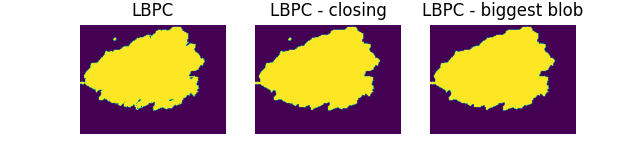
\includegraphics[scale=0.8]{images/segmentation/LBPC-1.png}
    
\includegraphics[scale=0.8]{images/segmentation/LBPC-2.png}
    
\includegraphics[scale=0.8]{images/segmentation/LBPC-3.png}
    \caption{SegNet followed by LBPC and transformation methods morphology closing and finding the biggest blob.}\label{SegNet-examples}
\end{figure}

Otsu threshold is a versatile automatic image thresholding technique meant to separate each pixel between two classes of foreground or background. One of the benefits of this method is that it does not require any training data. The equation \ref{otsu} (within-class variance) describes splitting weights of $w_0(t),w_1(t)$, which are the probabilities divided by the threshold $t$, between 0 and 255. Furthermore, $\sigma_1^2$ and $\sigma_0^2$ are variances of these two classes. The class probability $w$ is computed from the histogram in figure\ref{otsu2}, which is an intensity histogram describing the colour distribution in an image. Measuring the values above and below the generated thresholds splits the image into two classes.

\begin{equation}
\sigma_w^2(t) = w_0(t)\sigma_1^2(t) + w_1(t)\sigma_2^2(t)
\end{equation}\label{otsu}

The histogram was split into two segments with the threshold $t$ of 138 and the corresponding pixel locations to the histogram segment the skin lesion into two classes. Image morphology closing was applied to fill gaps that the threshold missed. On other occasions, the segmentation missed the skin lesion because of a similar colour between the skin and the skin lesion. It might be beneficial to combine Otsu with SegNet to improve its accuracy while producing a border cut-off. Figure\ref{otsu2} describes the difference between otsu and SegNet.

\begin{figure}
\centering
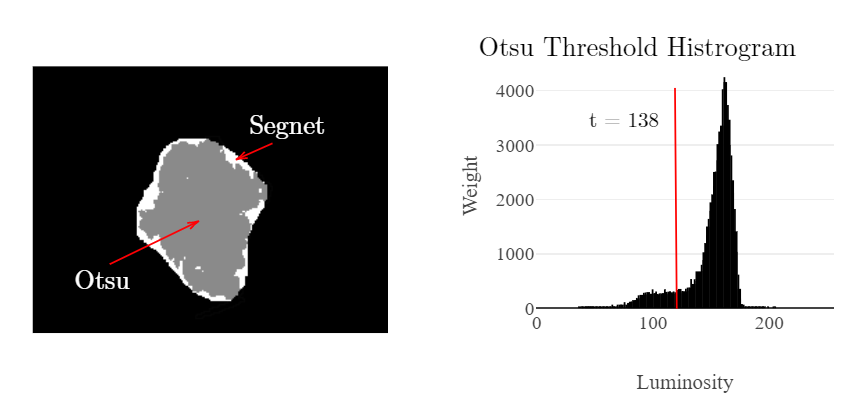
\includegraphics[scale=0.7]{images/otsu3.png}
\caption{Otsu thresholding alongside ground-truth mask, where grey Otsu and white is SegNet. The bar chart shows the histogram with an otsu threshold of 138.}\label{otsu2}
\end{figure}

\subsection{Local Binary Pattern clustering (LBPC) Segmentation}
Local Binary Patterns (LBP) is a texture descriptor commonly used for augmenting the image improving classification accuracy\cite{Pereira2020, Kaya2016}. First, equation\ref{eq1} calculates each pixel, where $p$ (equal to 8) is the number of neighbouring pixels compared to the centre of $c$, and the radius of $r$ from the centre. Next, shown in equation\ref{eq2} each value is subtracted counter-clockwise with the centre value and compared to function $S$ where each $gp - gc$, if more than or equal to 0, is equal to 1, and less than 0 is equal to 0. Next, add corresponding values equal to 1 of $gp$ together, changing the centre value, ignoring values of 0. Next, applying a Gaussian kernel of 13-pixel iterations and a standard deviation of 3 removes smaller features that interfere with the segmentation. Finally, applying k-means with a value of 2 subtracts the greyscale and segments the skin lesion from the skin.

\begin{equation} \label{eq1}
LBP(gp_x, gp_y) = \mathlarger{\sum}_{p=0}^{P-1}s\big(gp - gc)2^p
\end{equation}

\begin{equation} \label{eq2}
s\big(x) = 
\begin{cases}
1,\:\:x\geq\:0; \\
0,\:$otherwise$.
\end{cases}
\end{equation}

Figure \ref{fractal1} demonstrates the segmentation of two skin lesions, one with an irregular border and another with a regular border. LBPC is applied to both skin lesions, followed by Gaussian blurring and morphology closing to remove dots. The result is an improved border cut-off compared to the ground truth in the Ph$^2$ dataset with more corners and ledges. This technique will improve accuracy for measuring border irregularity\cite{Pereira2020}.

\begin{figure}
\centering
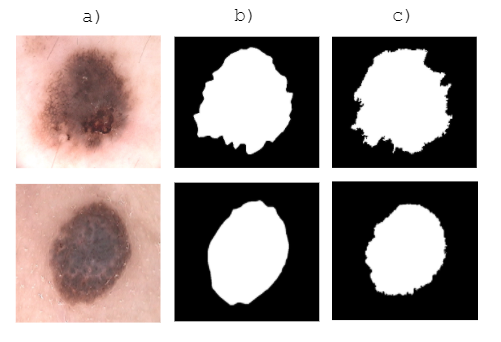
\includegraphics[scale=1.2]{images/borders.PNG}
\caption{Local Binary Pattern Clustering (LBPC) showing the a) original image, b) ground-truth, and c) LBPC. LBPC successfully exaggerates the border cut-off on the skin lesions with regular and irregular borders} 
\end{figure}\label{fractal1}

Validating LBPC is not expected because the goal is to exaggerate the border to improve the classification process of ABCD rules, which it does successfully\cite{Pereira2020, Kaya2016}. For example, the segmentation might not match dataset segmentations but is still essential to classifying ABCD rules. Furthermore, many datasets lack expert border segmentation, an accurate border cut-off between the skin and skin lesions, so comparisons are not always possible.

\section{Issues}
One issue with this technique is the overreliance on the size of the skin lesion. For it to function properly it needs to have a certain amount of skin and skin lesion for the segmentation to be possible. This leads to some concern when it comes to melanoma which is frequently larger and takes up more space in the image. This means that the accuracy of LBPC is in question for larger skin lesions. Here are some examples where the algorithm failed:

\begin{figure}
    \centering
    %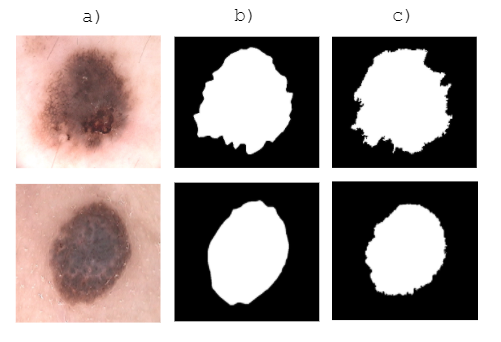
\includegraphics[scale=1.2]{images/borders.PNG}
    \caption{} 
\end{figure}\label{lbpc-issues}

\subsection{Results}
%Measure accuracy
Overall the accuracy of the techniques demonstrates that SegNet is the most reliable technique. However, comparing the techniques in \ref{} we can demonstrate that it produces a smudge effect and fails to capture the border cut-off from the skin lesion, but it is successful at finding the location of the skin lesion.

Both statistical models of LBPC and Otsu threshold generated an accurate border cut-off between the skin and the skin lesion As previously mentioned, measuring the border cut-off and exaggerating irregular borders are helpful when calculating the ABCD rules. 

It might be beneficial to combine SegNet and LBPC using SegNet to find the skin lesions' location, followed by adjusting the border cut-off using LBPC. A similar technique using the Otsu threshold and Segnet is described by Riaz et al.\cite{Riaz2019}.


\subsection{SegNet}

\subsection{LBPC}

\subsection{Otsu}

\subsection{Joint Segnet comparison}


\section{Experimental Results}
%Show that regardless of segnet being better that the other techniques still have a better border cut-off improving border irregulrity detection
This section includes a simple border analysis technique called fractal box-counting to assess the benefits of using different segmentation algorithms with accurate border cut-offs.

To prove the usefulness of segmentation techniques with an accurate border cut-off a technique developed by Ali\cite{Ali2020b} is implemented that utilises machine learning with extracted data including Zernike moments, fractal box-counting, and convexity measurements. Fractal box-counting is used to measure the irregularity of the border.

The fractal box-counting technique is a commonly employed technique for analysing fractal properties. It involves dividing a fractal object or pattern into a grid of equally sized boxes and counting the number of boxes that contain a portion of the fractals. The process is repeated with different box sizes until the boxes until the relationship between the box sizes and the number of boxes is analysed determining the fractal dimension\cite{Hamburger1996}. Essentially a more complicated border with corners and convexes will have more boxes and therefore a higher fractal score, than for example a border with smooth corners and edges which has a lower score. This should provide some evidence of the usefulness of an accurate border.

\subsection{Issues}
Although these techniques are massively accurate they are trained and tested against datasets (ISIC 2018) containing a mixture of approximate segmentation masks and expert segmentation masks. 

As mentioned in the previous section the ISIC 2018 dataset contains a mixture of approximate borders and expert borders. The statistical algorithms (otsu, LBPC) generate an accurate border cut-off and would have better accuracy for expert borders, but worse for approximate borders. The opposite is true for deep learning algorithms (U-net, SegNet) where they produce approximate borders and should ideally be tested against approximate borders.

Considering these problems to better assess the quality of algorithms the ISIC 2018 dataset could be split into different border types. This still has its issues because the border cut-off is subjective and where the skin lesion and skin end is still up to debate. The reason for extracting the border cut-off from the skin lesions is for better analysis of ABCD rules. So, both border types are assessed using fractal box counting, where the value should increase with more complex borders. 

Figure \ref{seg-expert} shows approximate borders are a rough estimation of skin lesion area and expert segmentation masks fit the skin lesion tighter representing border features. The mixture of images results in produced borders from many deep learning techniques having an inaccurate border cut-off border, whilst appearing accurate when tested against datasets. The ISIC 2018 dataset has a mixture of approximate segmentation masks and expert borders, which is not enough to train deep learning algorithms. Furthermore, the images are also shrunk as part of the deep learning process, which in turn loses smaller features that are significant when analysing borders. Various hybrid techniques have been developed using statistical algorithms active contouring-based segmenatation\cite{Riaz2019}, LBPC and others for border adjustment including u-otsu and edge-imfill. Specifically, u-otsu has been previously used to adjust the borders of melanoma to create expert borders\cite{}.

As shown in figure \ref{seg-expert} expert borders are tighter to the area of the skin lesion and approximate borders are the area of the lesion. Images have either approximate borders or expert borders and no others in the ISIC 2018 dataset, measurements are likely skewered because of the variation in types of borders.

%Show that LBPC sometimes fails at finding the skin lesion
The segmentation algorithms encountered some issues, whilst the best of the techniques was SegNet with an 85\% accuracy when relating to the ISIC 2019 dataset. However, as previously mentioned the segmentation masks have poor border cut-off stunting features that are useful for finding border irregularities. 

In contrast, LBPC and U-Otsu algorithms effectively identify the border cut-off of the skin lesion, which isn't properly represented in the ISIC 2019 dataset. But, it sometimes fails to find the skin lesion or does not detect anything. 

Both techniques appear to have downfalls making them less effective for use for analysing ABCD rules. It would be beneficial to find the approximate area of the skin lesion using SegNet and followed by LBPC to find the border cut-off.

\section{Joint Neural network and statistical model approach}
%Combine techniques together to get the area of the border

Combining both SegNet and LBPC improves the accuracy.
